\section{Background on Cracking}
\label{sec:background}


\subsection{Database cracking}
Cracking has been studied originally in the context of main-memory
column-stores as a simple adaptive indexing approach on \emph{one-dimensional}
data \cite{DBLP:conf/cidr/IdreosKM07} integrating data reorganization with query processing. 
For every dimension or column accessed in the workload a partial index is 
built incrementally during query processing.
The fix-point of one-dimensional database cracking is sorting the queried columns.


The data structures needed to support an end-to-end database 
cracking architecture are the following.
\begin{itemize}
\item A copy of the original column, namely \emph{cracker column}, which is
reorganized during query processing leaving the original column in the same
status.
\item A \emph{cracker index} to maintain the information about the indexed 
parts of the \emph{cracker column}.
\item A copy of the row ids used used as a \emph{map} for tuple reconstruction.
\end{itemize}

The first time a column $\mathtt{A}$ is accessed by a query, the system 
creates the cracker column $\mathtt{A_{CRK}}$,
and initializes the respective cracker index. Subsequent queries on
$\mathtt{A}$ incrementally build the cracker index by
reorganizing the underlying data into logical partitions using the query
predicates as pivots. The information about the values that are contained in
each partition is maintained in the cracker index, which is an $AVL$-tree. The
$AVL$-tree navigates subsequent queries to the correct partitions in order to
find the qualifying tuples. The qualifying tuples lay in a contiguous space in
memory which is returned as a result. To be able to reconstruct the original
tuples, the map with the original row ids is also maintained and reorganized
together with the cracker column.
Since the reorganization of the index is part of the select
operator, \emph{Database Cracking} can be seen as an alternative
implementation of scanning \cite{efficient_cracking}. 


Figure~\ref{fig:adaptive} shows how the data and the index is reorganized after
processing two subsequent queries. The first query requests values between $26$
and $31$. While searching attribute $\mathtt{Age}$ for the qualifying tuples,
the cracker column $\mathtt{Age_{CRK}}$ is reorganized such that values less than or equal to $26$ are gathered in the
first partition, values between $26$ and $31$ are gathered in the second
partition and values greater than or equal to $31$ are gathered in the third partition.
The second partition contains all qualifying values in contiguous memory and is
returned as the result. Thus, after processing the first query, values are
partitioned in three pieces. To answer the second query we navigate to the
first and the second partition (the third partition is entirely excluded from the
result) using the \emph{cracker index}. In order to find the qualifying tuples,
e.g., values between $24$ and $29$, values in the first and in the second 
partition are reshuffled using $24$ and $29$ respectively as pivots. The values
in partitions $2$ and $3$ are returned as a result. The more queries 
processed, the more partitions are created and thus subsequent queries have to
touch less and less data. When partitions are sorted or they reach a minimum size,
 found to be equal to half of the $L2$ cache size, then no further cracking 
actions take place.

\begin{figure}[t]
\begin{center}
\vspace*{3\baselineskip}
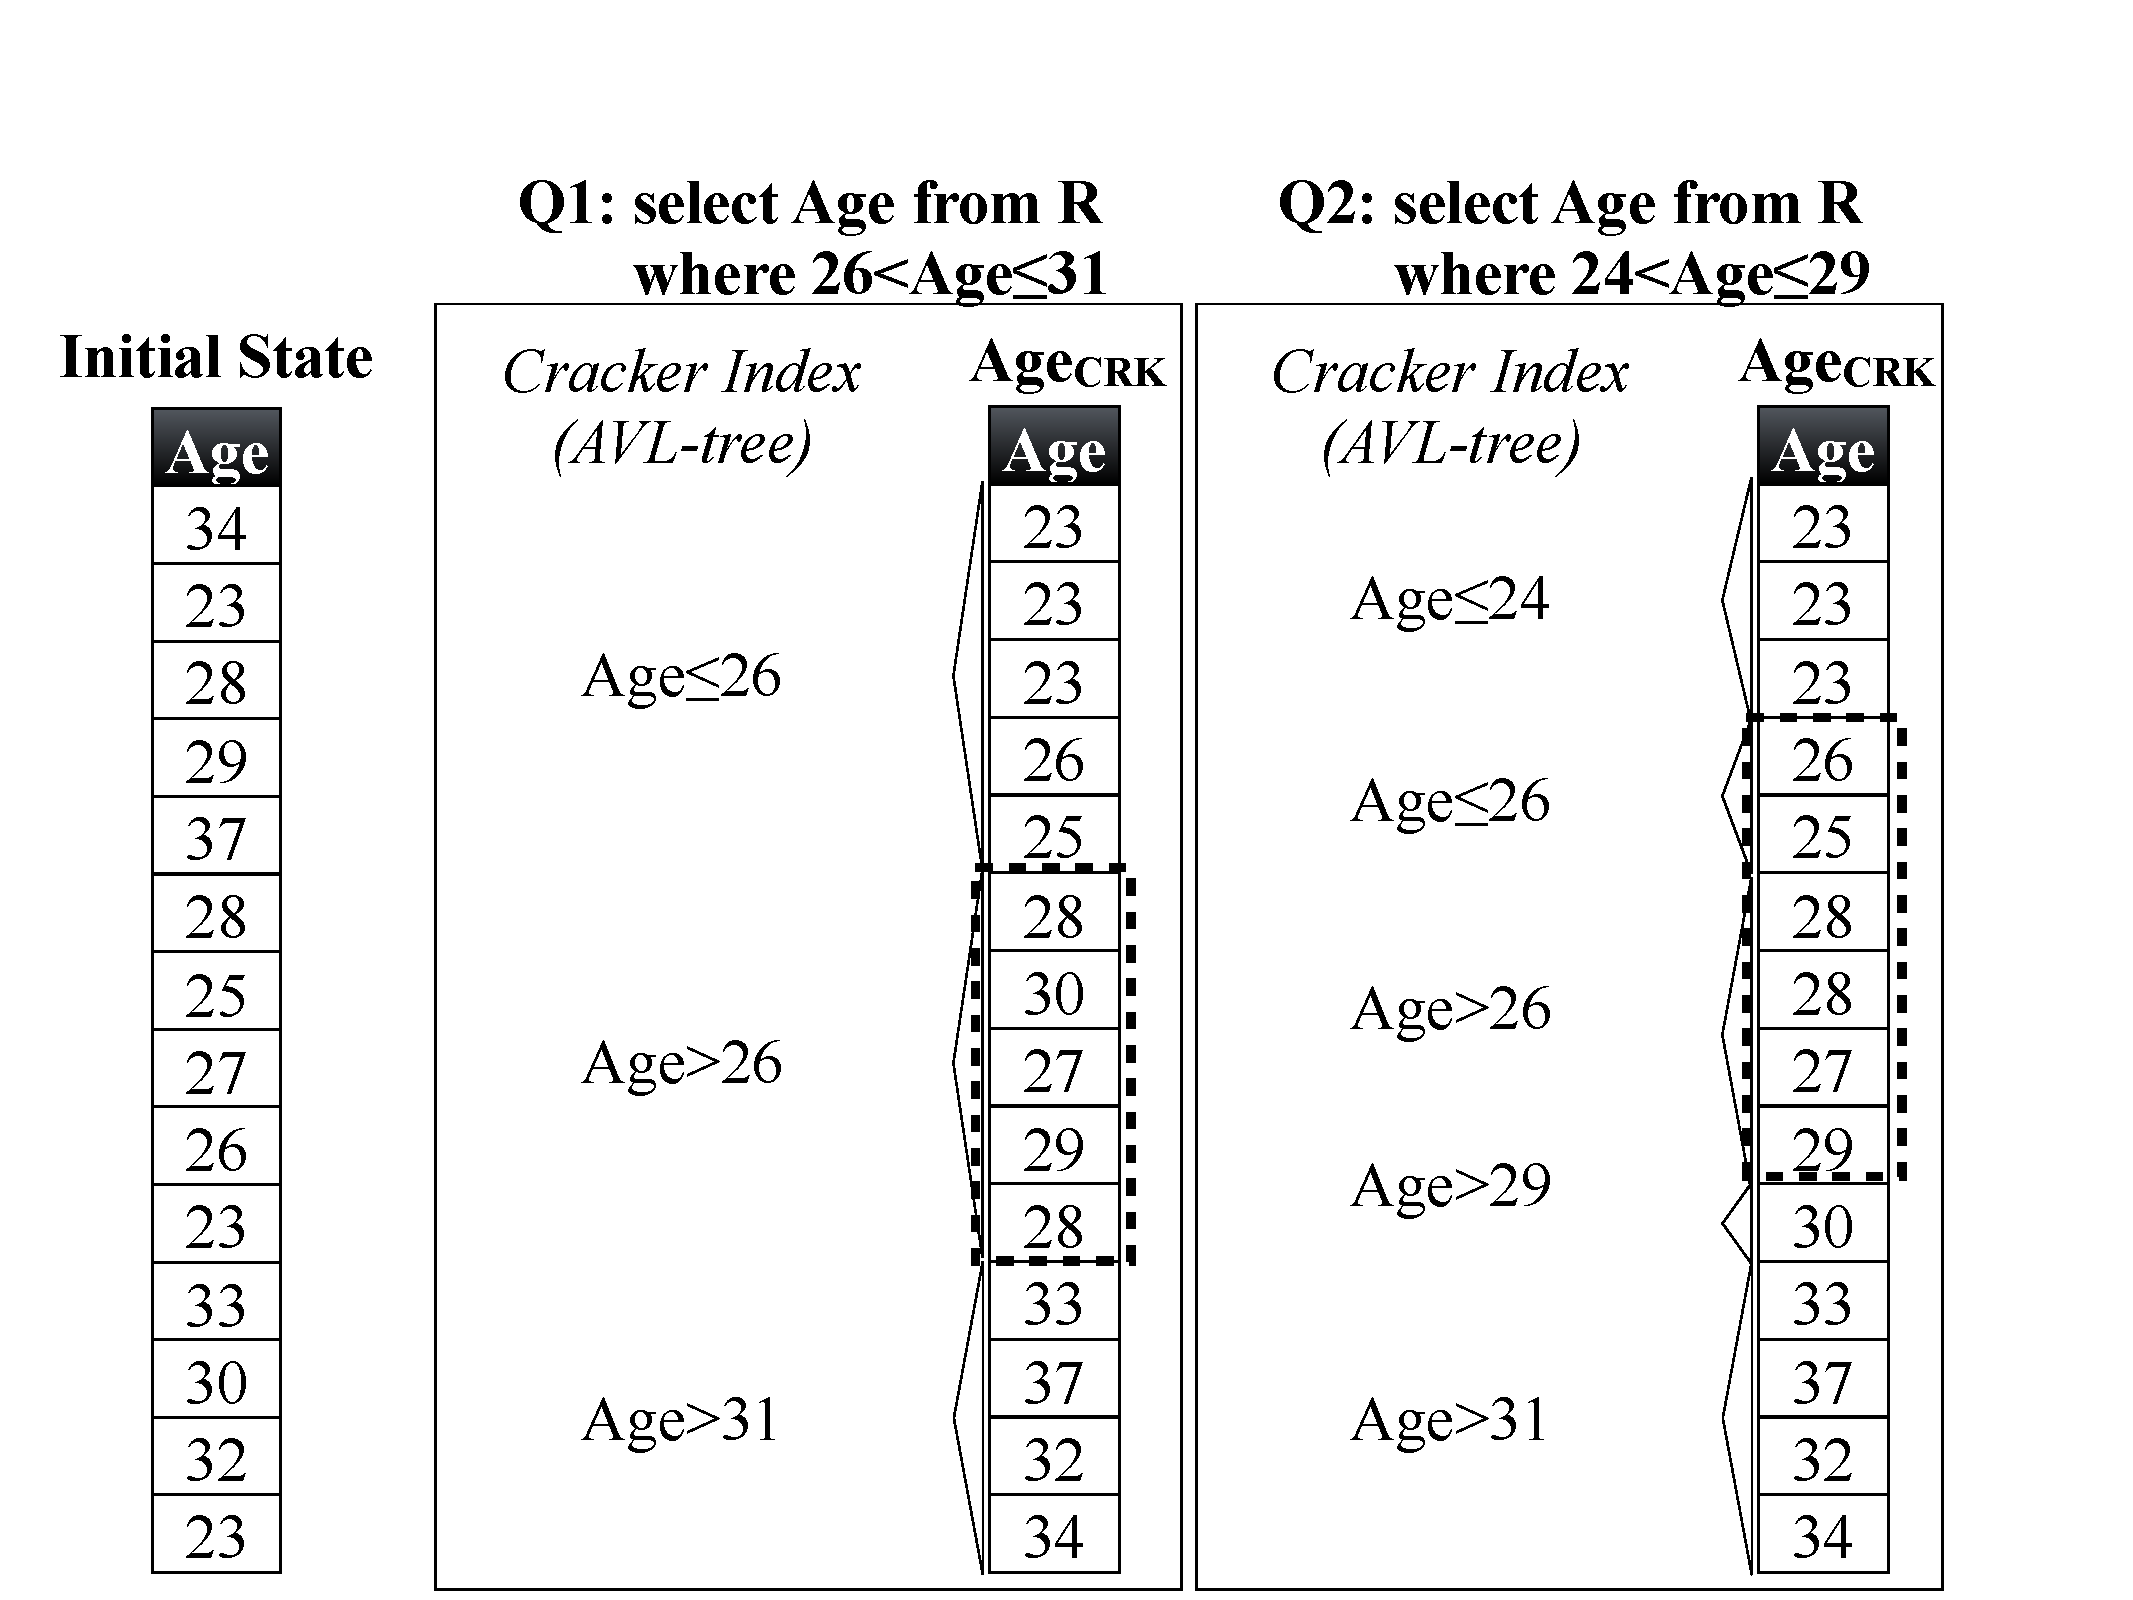
\includegraphics[trim=0cm 1cm 0cm 9cm, width=\columnwidth]{Figures/cracking_copy}
\caption{Database Cracking.}
\label{fig:adaptive}
\end{center}
\end{figure}

Database cracking has been shown to work for many core database architecture issues 
such as updates \cite{DBLP:conf/sigmod/IdreosKM07}, multi-selection/ projection queries \cite{DBLP:conf/sigmod/IdreosKM09}, concurrency control \cite{DBLP:journals/pvldb/GraefeHIKM12, CrackingTransactions}, partition-merge-like logic \cite{DBLP:conf/edbt/GraefeK10,DBLP:journals/pvldb/IdreosMKG11}. 
Stochastic database cracking \cite{DBLP:journals/pvldb/HalimIKY12} shows how to be robust on various query workloads.
Finally, \cite{IndexingKeys} shows how adaptive indexing can apply to key columns.


\begin{figure}[t]
\begin{center}
\vspace*{3\baselineskip}
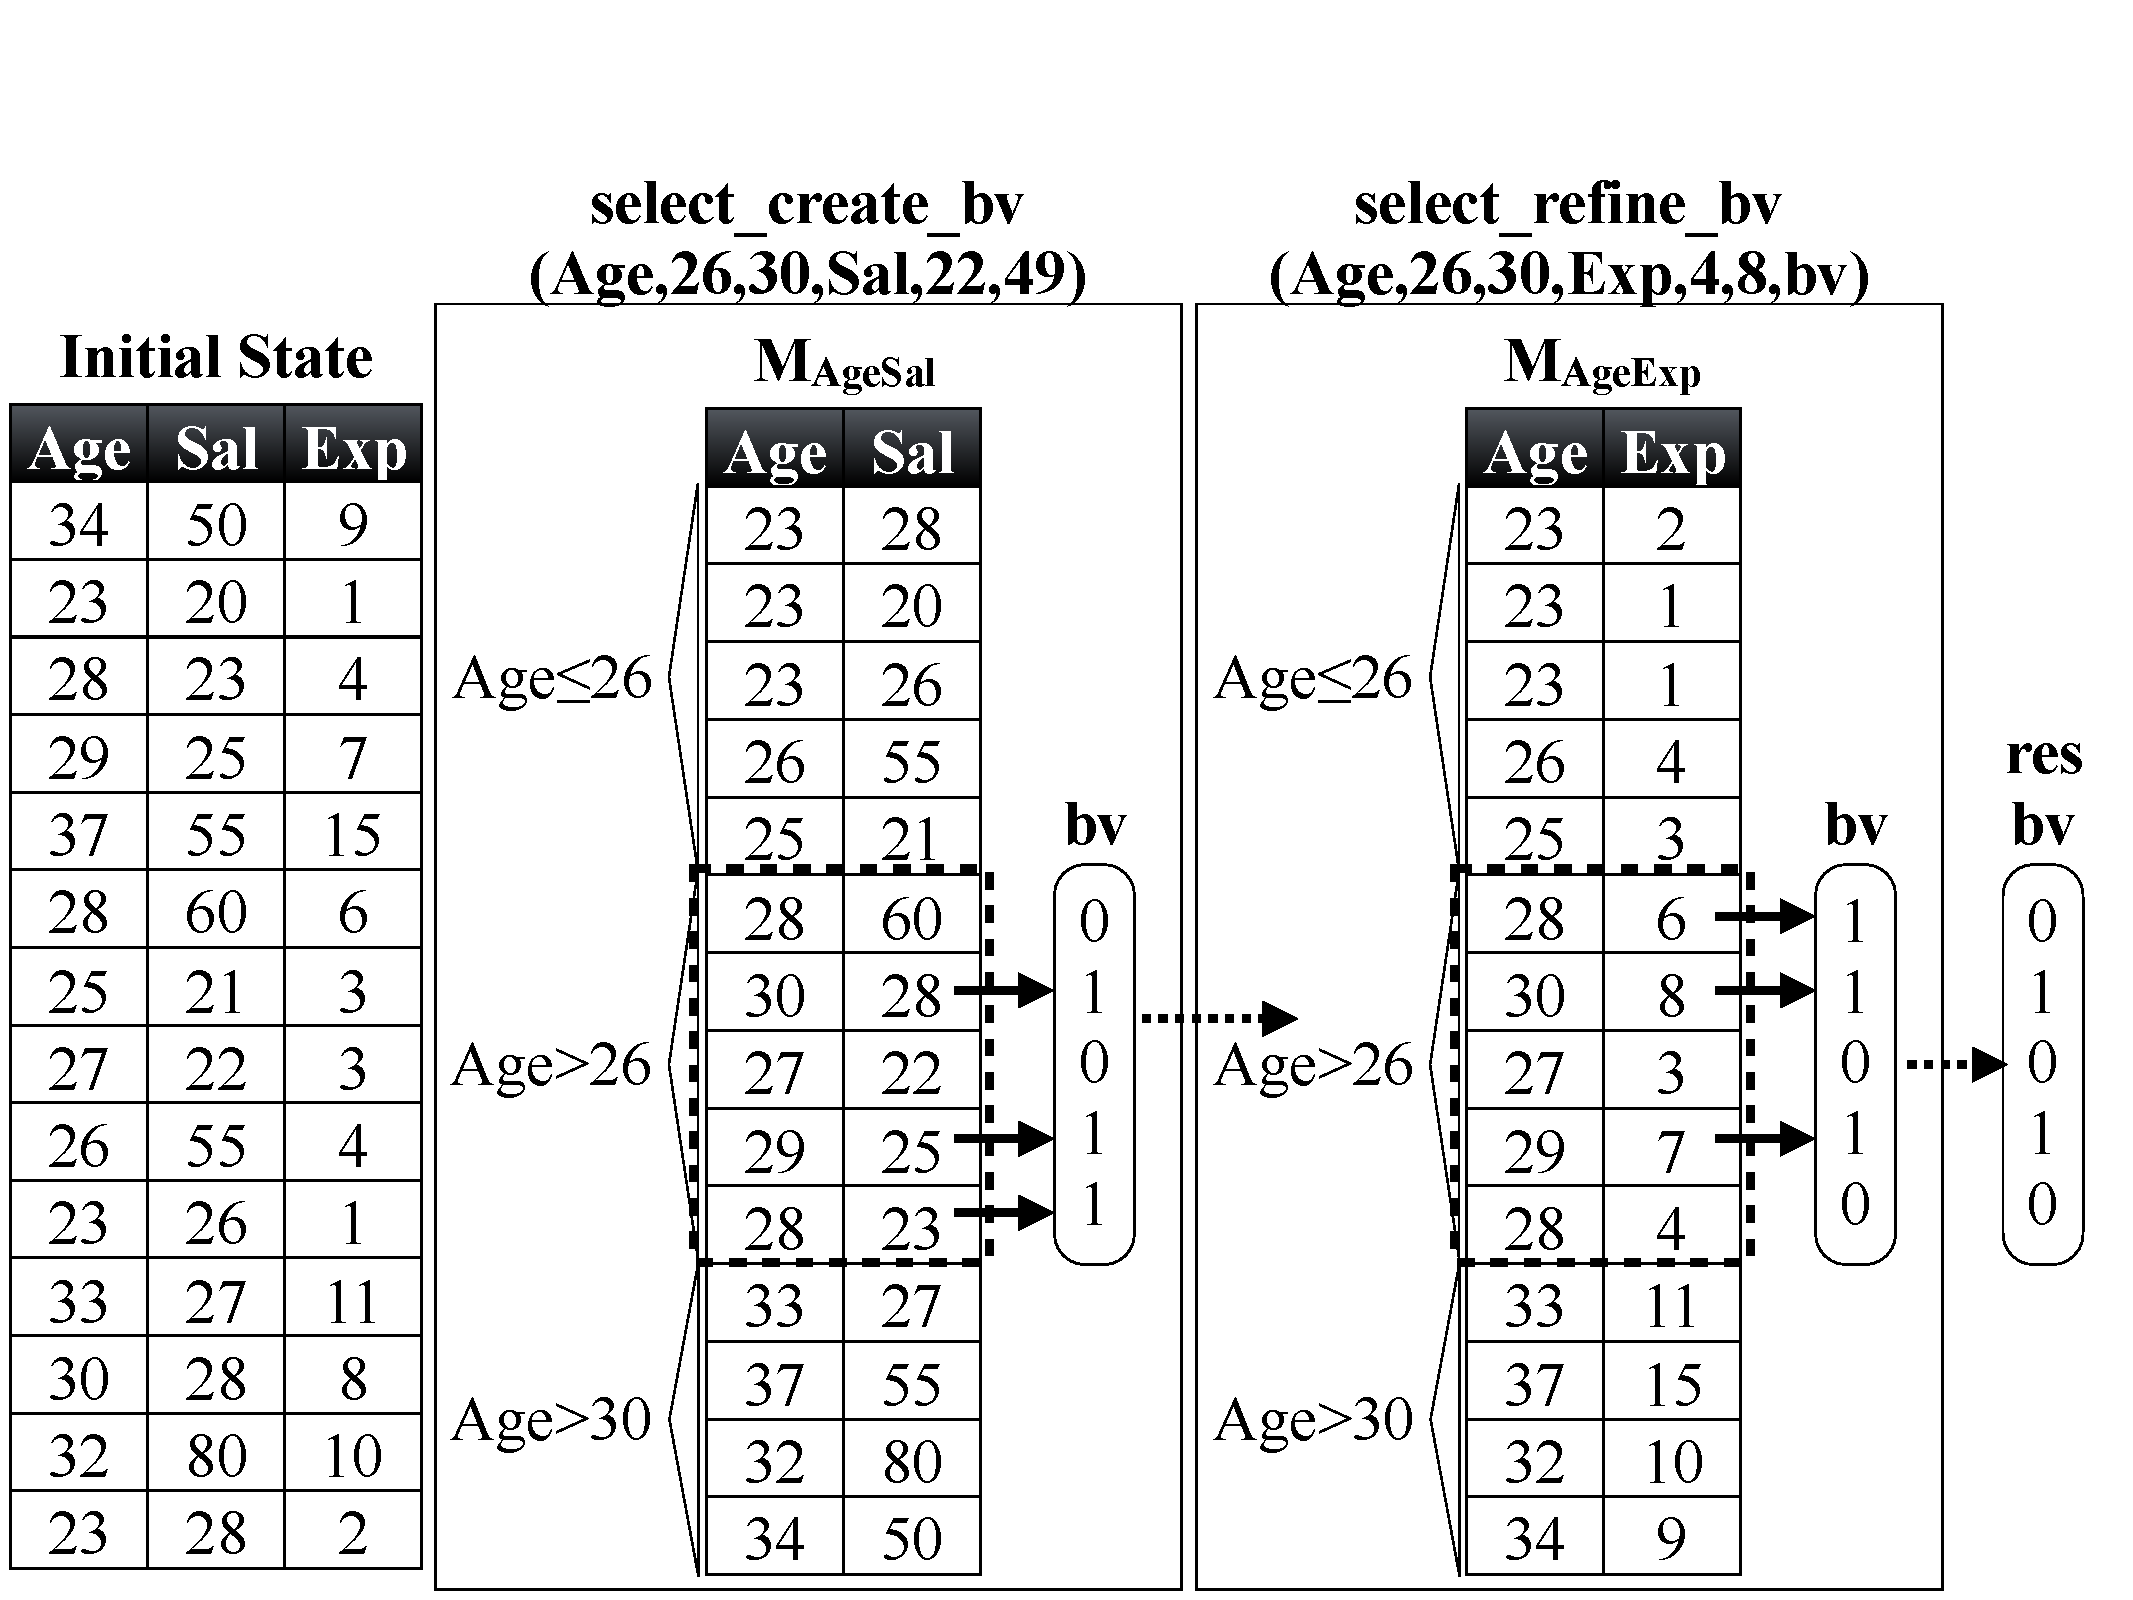
\includegraphics[trim=0cm 1cm 0cm 9cm, width=\columnwidth]{Figures/sideways_cracking}
\caption{Sideways Cracking.}
\label{fig:sideways}
\end{center}
\end{figure}

\subsection{Sideways cracking}
Sideways cracking handles the tuple reconstruction for queries that
include selections and/or projections on multiple columns 
\cite{DBLP:conf/sigmod/IdreosKM09}, while \emph{partial sideways cracking} \cite{DBLP:conf/sigmod/IdreosKM09} 
reduces the storage overhead of sideways cracking.
Sideways cracking maintains and incrementally reorganizes the following data structures.

\begin{itemize}
\item \emph{Cracker maps} which consist of two columns that appear in the same query. 
A cracker map $\mathtt{M_{Ax}}$ is cracked only on $\mathtt{A}$.
The tuples of $\mathtt{x}$ are reorganized together with the tuples of
$\mathtt{A}$ to maintain the alignment between these two attributes.
All cracker maps that use $\mathtt{A}$ as the cracking column belong to 
\emph{map set $\mathtt{S_A}$}. 
\item A \emph{cracker index} (AVL-tree) for each cracker map $\mathtt{M_{Ax}}$ that maintains the information about $\mathtt{A}$.
\item A \emph{cracker tape} for each map set $\mathtt{S_A}$ that logs all cracks on $\mathtt{A}$.
Different cracker maps of the same map set use the cracker tape on demand to ensure alignment.
\item Bit vectors with bits set for the tuples that qualify both selection predicates of both columns of the cracker map.
A conjunction/disjunction of the bit vectors is used to produce the final result.
\end{itemize}

Figure~\ref{fig:sideways} shows how the data and the index is reorganized after
processing a query $\mathtt{Q_{1}}$, which includes a multiple selection and projection
on attributes $\mathtt{Age}$, $\mathtt{Salary}$ and $\mathtt{Experience}$.
To answer this query we need two cracker maps, i.e., $\mathtt{M_{AgeSal}}$ and $\mathtt{M_{AgeExp}}$.
Both maps are reorganized based on the selection predicate on $\mathtt{Age}$.
Tuples with $\mathtt{Age}$ value less than or equal to $26$ are gathered in the
first partition, values between $26$ and $31$ are gathered in the second
partition and values greater than or equal to $31$ are gathered in the third partition.
A cracker index for every map maintains the partitioning information.
While reorganizing $\mathtt{Age}$, $\mathtt{Salary}$ and $\mathtt{Experience}$ are reorganized too to ensure alignment.
After reorganizing $\mathtt{M_{AgeSal}}$ a bit vector has a bit set for all these tuples that qualify the selection predicates both on $\mathtt{Age}$ and $\mathtt{Salary}$.
Similarly, another bit vector has a bit set for all these tuples that qualify the selection predicates both on $\mathtt{Age}$ and $\mathtt{Experience}$.
The conjunction of the two bit vectors can be used to produce the final result.

Although sideways cracking handles queries with selections or projections on multiple attributes, it does so by reorganizing only one dimension at a time.
